\documentclass{beamer}
\usepackage[utf8]{inputenc}
\usepackage[T1]{fontenc}
\usepackage{lmodern}
\usepackage{ngerman}
\usepackage{bibgerm}
\usepackage{color}
\usepackage{graphicx}
\usepackage{pstricks}

\mode<presentation>  {
  \usetheme{Warsaw}
  \useoutertheme{miniframes}
  \setbeamertemplate{navigation symbols}{}
}

\newcommand{\defaultscale}{0.5}
\newcommand{\pfeil}{\item[$\Rightarrow$]}
\newcommand\ato{\rightarrow} %Morphismen

\newcommand{\sexp}{S"=Expression}
\newcommand{\sexps}{S"=Expressions}
\newcommand{\cgen}{Code"=Generierung}
\newcommand{\cpp}{C\texttt{++}}
\newcommand{\mprog}{Metaprogrammierung}

\title[\mprog{}]{Prototyp eines \sexp{}-basierten Rahmenwerks für
  sprachübergreifende \mprog{}}
\subtitle{Diplomarbeit}
\author[Benjamin Teuber]{Benjamin Teuber\\ Erstbetreuer: Daniel
  Moldt\\ Zweitbetreuer: Leonie Dreschler-Fischer}
\date{\today}
\institute{TGI-Oberseminar\\
  Universität Hamburg\\ 
  Fakultät für Mathematik, Informatik und Naturwissenschaften\\
  Department Informatik}

\begin{document}

\section{Einführung}
\subsection{Einführung}

\maketitle

\AtBeginSubsection{
\begin{frame}
\begin{center}
\structure{\Huge \insertsubsection}
\end{center}
\end{frame}
}

\begin{frame}{Themengebiet}
  \begin{itemize}
  \item Thema: \mprog{}
    \begin{itemize}
    \item Hier: \cgen{}
    \item Generative \mprog{}
    \item Statische \mprog
    \end{itemize}
  \item Starke Verbreitung
    \begin{itemize}
    \item Model-Driven Architecture
    \item Domain-Specific Languages
    \item Auch im AOSE-Projekt
    \end{itemize}
  \end{itemize}
\end{frame}

\begin{frame}{Motivation}
  \begin{itemize}
  \item Problem: Generator bauen ist aufwändig
  \item Viele Komponenten nötig
    \begin{itemize}
    \item Parser für Quellsprache
    \item Compiler in normaler Programmiersprache
    \item Templates für Zielsprache
    \end{itemize}  
  \item Wie können wir dies vereinfachen?
  \end{itemize}
\end{frame}

\begin{frame}{Zielsetzung}
  \begin{itemize}
  \item Entwurf eines eigenen Frameworks
  \item Davor:
    \begin{itemize}
    \item Vergleich bestehender Systeme
    \item Festlegen der Anforderungen
    \item Planung der Architektur
    \end{itemize}
  \end{itemize}
\end{frame}

\begin{frame}{Inhalt}
  \begin{itemize}
  \item Vorarbeit
    \begin{itemize}
    \item Vorhandene Technologien
    \item Anforderungen
    \end{itemize}
  \item MagicL
    \begin{itemize}
    \item Architektur
    \item Demo
    \end{itemize}
  \end{itemize}
\end{frame}

\begin{frame}{Anwendungsbeispiel}
  \begin{itemize}
  \item Slide, eine DSL für Vortragsfolien
  \item Wird nach Latex kompiliert
  \end{itemize}
  \begin{figure}
    \centering
    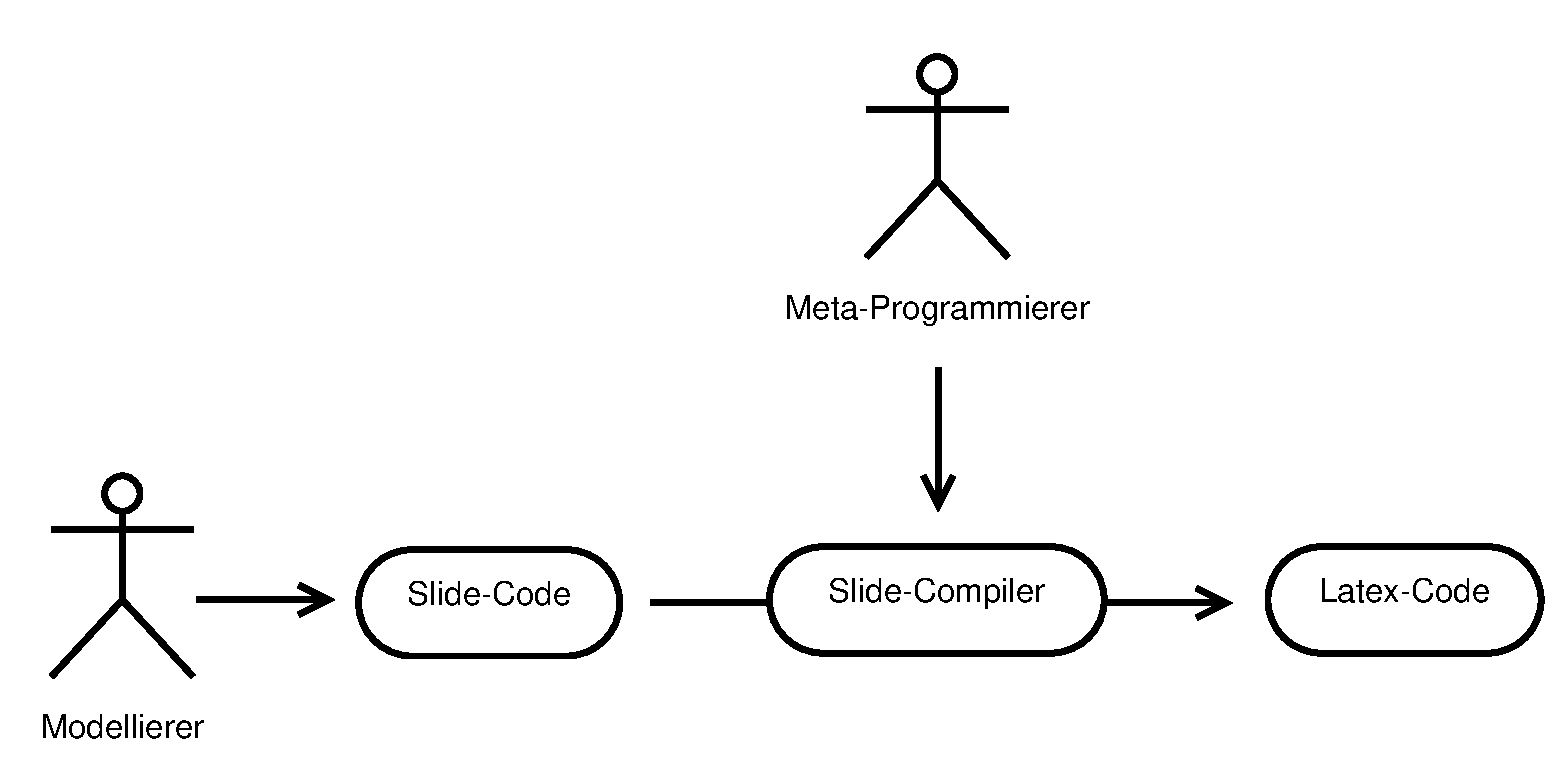
\includegraphics[scale=0.3]{images/flow_example_simple}
    \caption{Der Slide-Compiler}
  \end{figure}
\end{frame}

\section{Vorhandene Technologien}
\subsection{Vorhandene Technologien}

\begin{frame}{Unterschiede bestehender Werkzeuge}
  \begin{itemize}
  \item Modellrepräsentation
    \begin{itemize}
    \item Zeichenketten
    \item Objekte
    \item Bäume
    \end{itemize}
  \item Art der Code-Erzeugung
    \begin{itemize}
    \item Templates
    \end{itemize}
  \item Meta-Programmiersprache
    \begin{itemize}
    \item Mächtigkeit
    \item Ausdrucksstärke
    \end{itemize}
  \end{itemize}
\end{frame}

\begin{frame}{Modellrepräsentation}
  \begin{itemize}
  \item Zeichenketten
  \item Pro:
    \begin{itemize}
    \item Nötig für Serialisierung/Ausgabeformat
    \item Einfache Manipulation
    \item Universell
    \end{itemize}
  \item Contra:
    \begin{itemize}
    \item Low-Level
    \item Anfällig für Syntaxfehler
    \item Unstrukturiert
    \end{itemize}
  \end{itemize} 
\end{frame}

\begin{frame}{Modellrepräsentation (2)}
  \begin{itemize}
  \item Typisierte Objekte
  \item Pro:
    \begin{itemize}
    \item Typsicherheit
    \item Effizienz
    \end{itemize}
  \item Contra:
    \begin{itemize}
    \item Typdeklarationen nötig
    \item Manipulation komplizierter
    \end{itemize}
  \end{itemize} 
\end{frame}

\begin{frame}{Modellrepräsentation (3)}
  \begin{itemize}
  \item Ungetypte Bäume (XML, \sexps{}, JSON)
  \item Pro:
    \begin{itemize}
    \item Einfach
    \item Strukturiert
    \item Universell
    \item Sicherer als Strings
    \end{itemize}
  \item Contra:
    \begin{itemize}
    \item Nicht so sicher/effizient wie Objekte
    \end{itemize}
  \end{itemize} 
\end{frame}

\begin{frame}[fragile]{S-Expressions}
  \begin{itemize}
  \item Ein S-Expression ist entweder:
    \begin{itemize}
    \item Ein Atom, z.B. eine Zahl, ein String, eine Variable
    \item Eine Liste von S-Expressions in Notation 
    \item[] \texttt{($sexp_1$ $sexp_2$ .. $sexp_n$)}
    \end{itemize}
  \item Konvention: Knotenname an erster Stelle
  \item \textit{Strukturelle} Verarbeitung
  \item Minimale Komplexität (vgl. XML)
  \end{itemize}
\end{frame}

\begin{frame}[fragile]{S-Expressions (2)}
  \begin{block}{Beispiel: Folie in \sexps{}}
\begin{verbatim}
(slide
  (title My Slide)
  (image
    (source diagram.png)
    (caption This is a diagram))
  (list one two three))
\end{verbatim}
  \end{block}
  \begin{figure}
    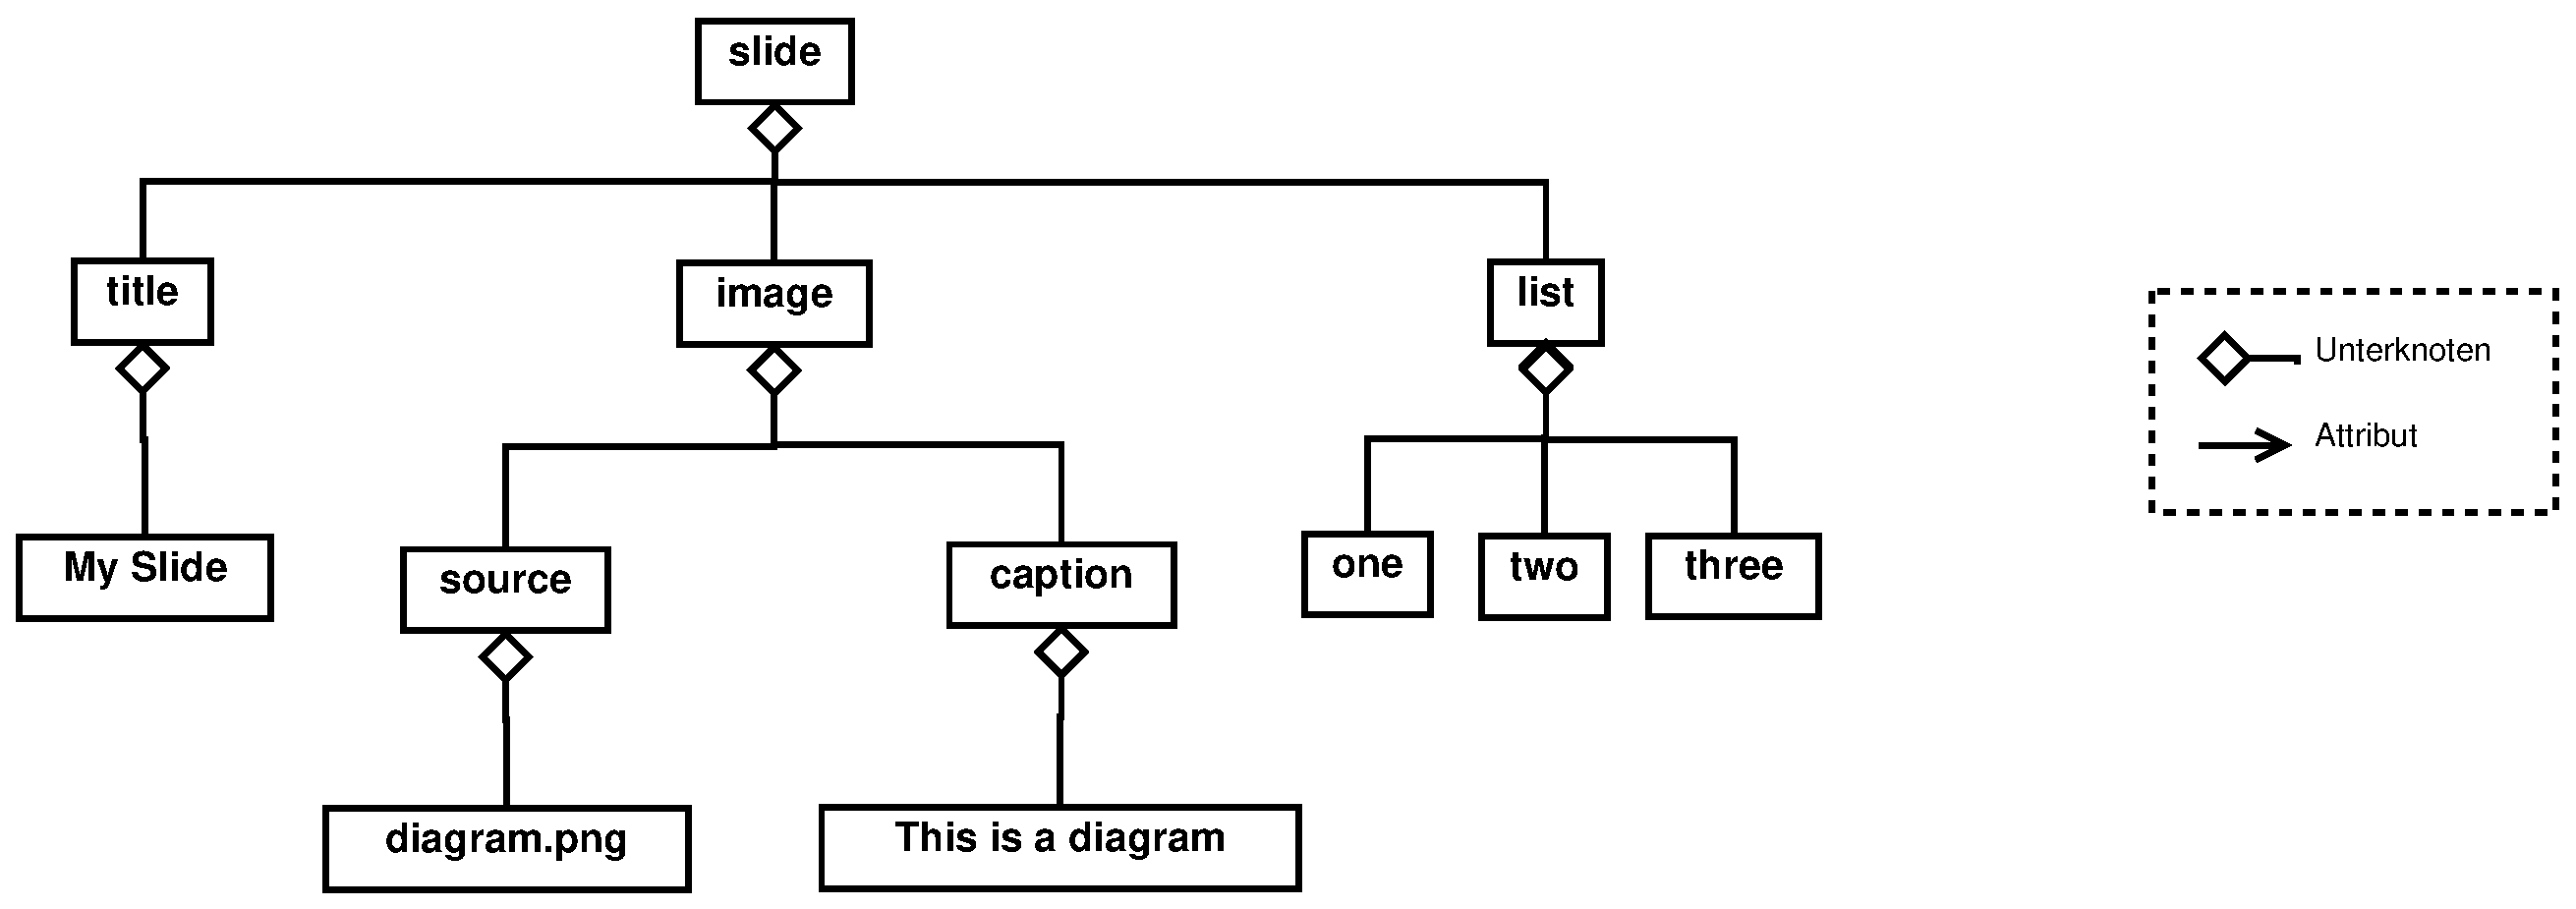
\includegraphics[scale=0.2]{images/model_slide_sexp}
  \end{figure}
\end{frame}

\begin{frame}[fragile]{Templates}
  \begin{itemize}
  \item Für Dokumenterzeugung genutzt
  \item ``Schablone mit Platzhaltern''
  \item Funktion: $\mathrm{input} \ato \mathrm{doc}$
  \item Typen $\mathrm{input}$ und $\mathrm{doc}$ variieren
  \end{itemize}
\end{frame}

\begin{frame}[fragile]{PHP}
  \begin{itemize}
  \item $\mathrm{Object}\ato\mathrm{String}$
  \item Zeichenketten problematisch da Fehleranfällig
  \item Komplette Programmiersprache
  \end{itemize}
\begin{verbatim}
<ul>
  <? foreach ($items as $item) {
       echo("<li>" . $item . "</li>");
     }
  ?>
</ul>
\end{verbatim}
\end{frame}

\begin{frame}[fragile]{XSL Transformation}
  \begin{itemize}
  \item $\mathrm{XML} \ato \mathrm{XML}$
  \item Mächtig, aber umständliche Syntax
    \begin{itemize}
    \pfeil Praxis: Komplexe Verarbeitung in externer
      Programmiersprache
    \end{itemize}
  \item Ermöglicht direkten Aufruf sowie Matching über XPath
  \item XPath: \verb+/book[@price>35]/title+
  \end{itemize}
\end{frame}

\begin{frame}[fragile]{XSLT (2)}

  \begin{block}{Eingabe}
\begin{verbatim}
<list>
  <item>foo</item>
  <item>bar</item>
  <item>baz</item>
</list>
\end{verbatim}
  \end{block}
  \begin{block}{Erwünschte Ausgabe}
\begin{verbatim}
<ul>
  <li>foo</li>
  <li>bar</li>
  <li>baz</li>
</ul>
\end{verbatim}
\end{block}
\end{frame}

\begin{frame}[fragile]{XSLT (3)}
\begin{verbatim}
<xsl:template match="/list">
  <ul>
    <xsl:for-each select="item">
      <li><xsl:value-of select="." /></li>
    </xsl:for-each>
  </ul>
</xsl:template>
\end{verbatim}
\end{frame}

\begin{frame}[fragile]{Lisp-Makros}
  \begin{itemize}
  \item $\mathrm{Sexp} \ato \mathrm{Sexp}$
  \item Metasprache $=$ Zielsprache $=$ Quellsprache $=$ Lisp
  \item ``Compiler-Plugins'' in kurzer, eleganter Notation
  \item Ermöglichen inkrementelle Erweiterung des Lisp-Compilers
    \begin{itemize}
    \item ``Embedded DSLs'' - in die ursprüngliche Sprache
      integriert
    \end{itemize}
  \item Template-Syntax:
    \begin{itemize}
    \item Quasiquote mit \texttt{`}  
    \item Unquote mit \texttt{,}  
    \end{itemize}
  \end{itemize}
\end{frame}

\begin{frame}[fragile]{Lisp-Makros (2)}
  \begin{block}{Eingabe}
\begin{verbatim}
(list
  (item foo)
  (item bar)
  (item baz))
\end{verbatim}
  \end{block}
  \begin{block}{Erwünschte Ausgabe}
\begin{verbatim}
(ul
  (li foo)
  (li bar)
  (li baz))
\end{verbatim}
  \end{block}
\end{frame}

\begin{frame}[fragile]{Lisp-Makros (3)}
  \begin{block}{Makro-Umsetzung in Common Lisp}
\begin{verbatim}
(defmacro item (text)
  `(li ,text))

(defmacro list (&rest items)
  `(ul ,@items))
\end{verbatim}
  \end{block}
\end{frame}

\section{Anforderungen}
\subsection{Anforderungen}

\begin{frame}{Lisp-inspiriertes Framework}
  \begin{itemize}
  \item \sexps{}
  \item Verallgemeinerte Makros
  \item Quasiquote
  \item Funktionale Metasprache
  \end{itemize}
\end{frame}

\begin{frame}{Unterstützte Modelltypen}
  \begin{itemize}
  \item \sexps{}
    \begin{itemize}
    \item Hauptfokus
    \item Standard für User-DSL
    \pfeil Parser entfällt 
    \end{itemize}
  \item Strings
    \begin{itemize}
    \item Parser
    \item Generatoren
    \item möglichst vom Benutzer versteckt
    \end{itemize}
  \item Objekte
    \begin{itemize}
    \item Für komplexere Berechnungen
    \item Typsicherheit
    \item Effizienz
    \end{itemize}
  \end{itemize}
\end{frame}

\begin{frame}{Unterstützte Modelltypen (2)}
  \begin{itemize}
  \item Alle drei Modelltypen verwendbar
    \begin{itemize}
    \item Als Eingabe
    \item Als Ausgabe
    \pfeil Neun Mögliche Compiler-Arten
    \end{itemize}
  \end{itemize}
  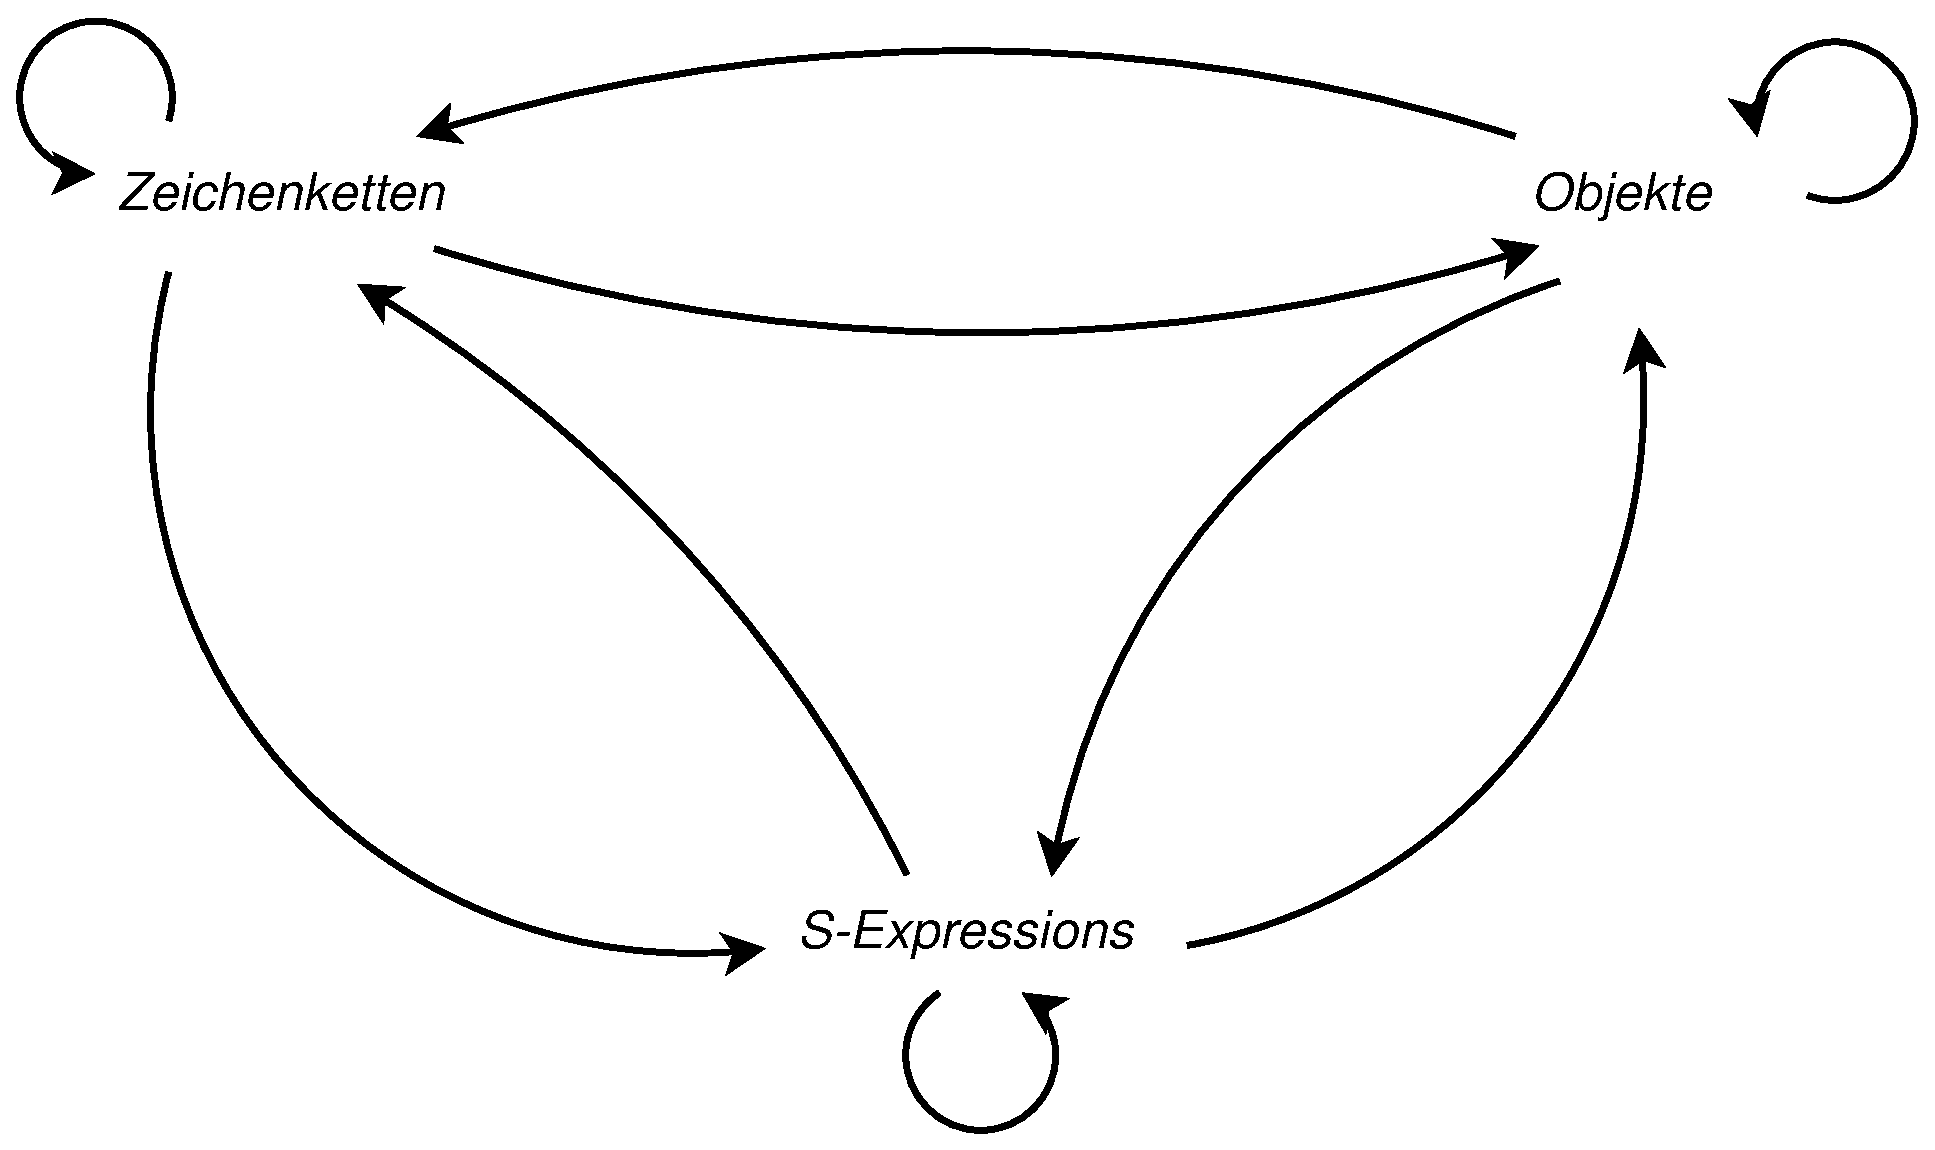
\includegraphics[scale=0.25]{images/magicl_model_poss}
\end{frame}

\begin{frame}[fragile]{\sexps}
  \begin{itemize}
  \item Einfachste Baumstruktur
  \item Hier: \textbf{Keine} weitere Syntax
  \pfeil Strings etc. müssen eingebettet werden
  \end{itemize}
\begin{verbatim}
(Str Hallo Welt)
\end{verbatim}
\end{frame}

\begin{frame}[fragile]{Quasiquote}
  \begin{itemize}
  \item Syntax angepasst
  \item beliebig viele Rückgaben möglich
  \end{itemize}
  \begin{block}{Quasiquote-Beispiele}
\begin{verbatim}
(' a b c d e)
(' (+ 3 (, x)))
(' (a b c (,@ list) h i))  
\end{verbatim}
  \end{block}
\end{frame}

\begin{frame}[fragile]{Verallgemeinerte Makros}
  \begin{itemize}
  \item Parser auf \sexps{}
  \item Aufruf genauer steuerbar
    \begin{itemize}
    \item Nicht nur Matching vom Knotennamen
    \item Lokale Makros möglich
    \item XPath
    \item EBNF
    \end{itemize}
  \end{itemize}
  \begin{block}{List-Makro in MagicL}
\begin{verbatim}
(macro "item"
  (>>^ take
       (fun text 
            (' (li (, text))))))  
\end{verbatim}
  \end{block}
\end{frame}

\section{Architektur}
\subsection{Architektur}

\begin{frame}{Programmiersprache}
  \begin{itemize}
  \item Haskell
  \item Funktional
  \item statische Typinferenz
  \item Kategorientheorie-Bibliotheken
  \end{itemize}
\end{frame}

\begin{frame}{Kategorientheorie}
  \begin{columns}
    \begin{column}{7cm}
      \begin{itemize}
      \item Sehr abstrakter Bereich der Mathematik
        \item Grundidee
          \begin{itemize}
          \item ``Rechnen mit Funktionstypen''
          \item Von Funktionen abstrahieren
          \pfeil flexible Verarbeitungsprozesse
          \end{itemize}
        \item visualisierbar
          \item Vergleich mit Petri-Netzen
            \begin{itemize}
            \item ``Punktfrei''
            \item Komposition überladbar
            \end{itemize}
      \end{itemize}
    \end{column}
    \begin{column}{4.5cm}
      \begin{center}
        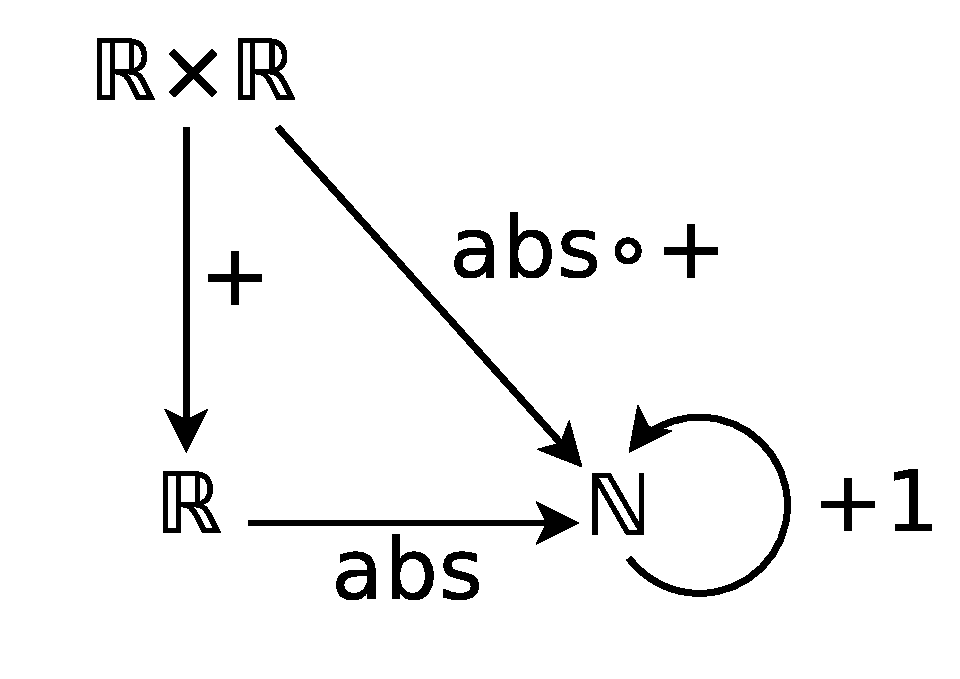
\includegraphics[scale=0.3]{images/cat_funs}
      \end{center}
    \end{column}
  \end{columns}
\end{frame}

\begin{frame}{Kategorien im MagicL}
  \begin{itemize}
  \item Überall genutzt
    \begin{itemize}
    \item Parser
    \item Compiler
    \item Diagramme in Doku
    \end{itemize}
  \item Umsetzung kategorientheoretischer Konzepte
    \begin{itemize}
    \item teils bereits in Haskell
    \item teils in Arrow-Bibliothek
    \end{itemize}
  \end{itemize}
\end{frame}

\begin{frame}{Unterstützung der Modelltypen}
  \begin{columns}
    \begin{column}{3.5cm}
      \begin{itemize}
      \item Strings
        \begin{itemize}
        \item Parser
        \item Generatoren
        \end{itemize}
      \item \sexps
        \begin{itemize}
        \item Parser
        \item Quasiquote
        \end{itemize}
      \item Objekte
        \begin{itemize}
        \item Funktionen
        \end{itemize}
      \end{itemize}
    \end{column}
    \begin{column}{8cm}
      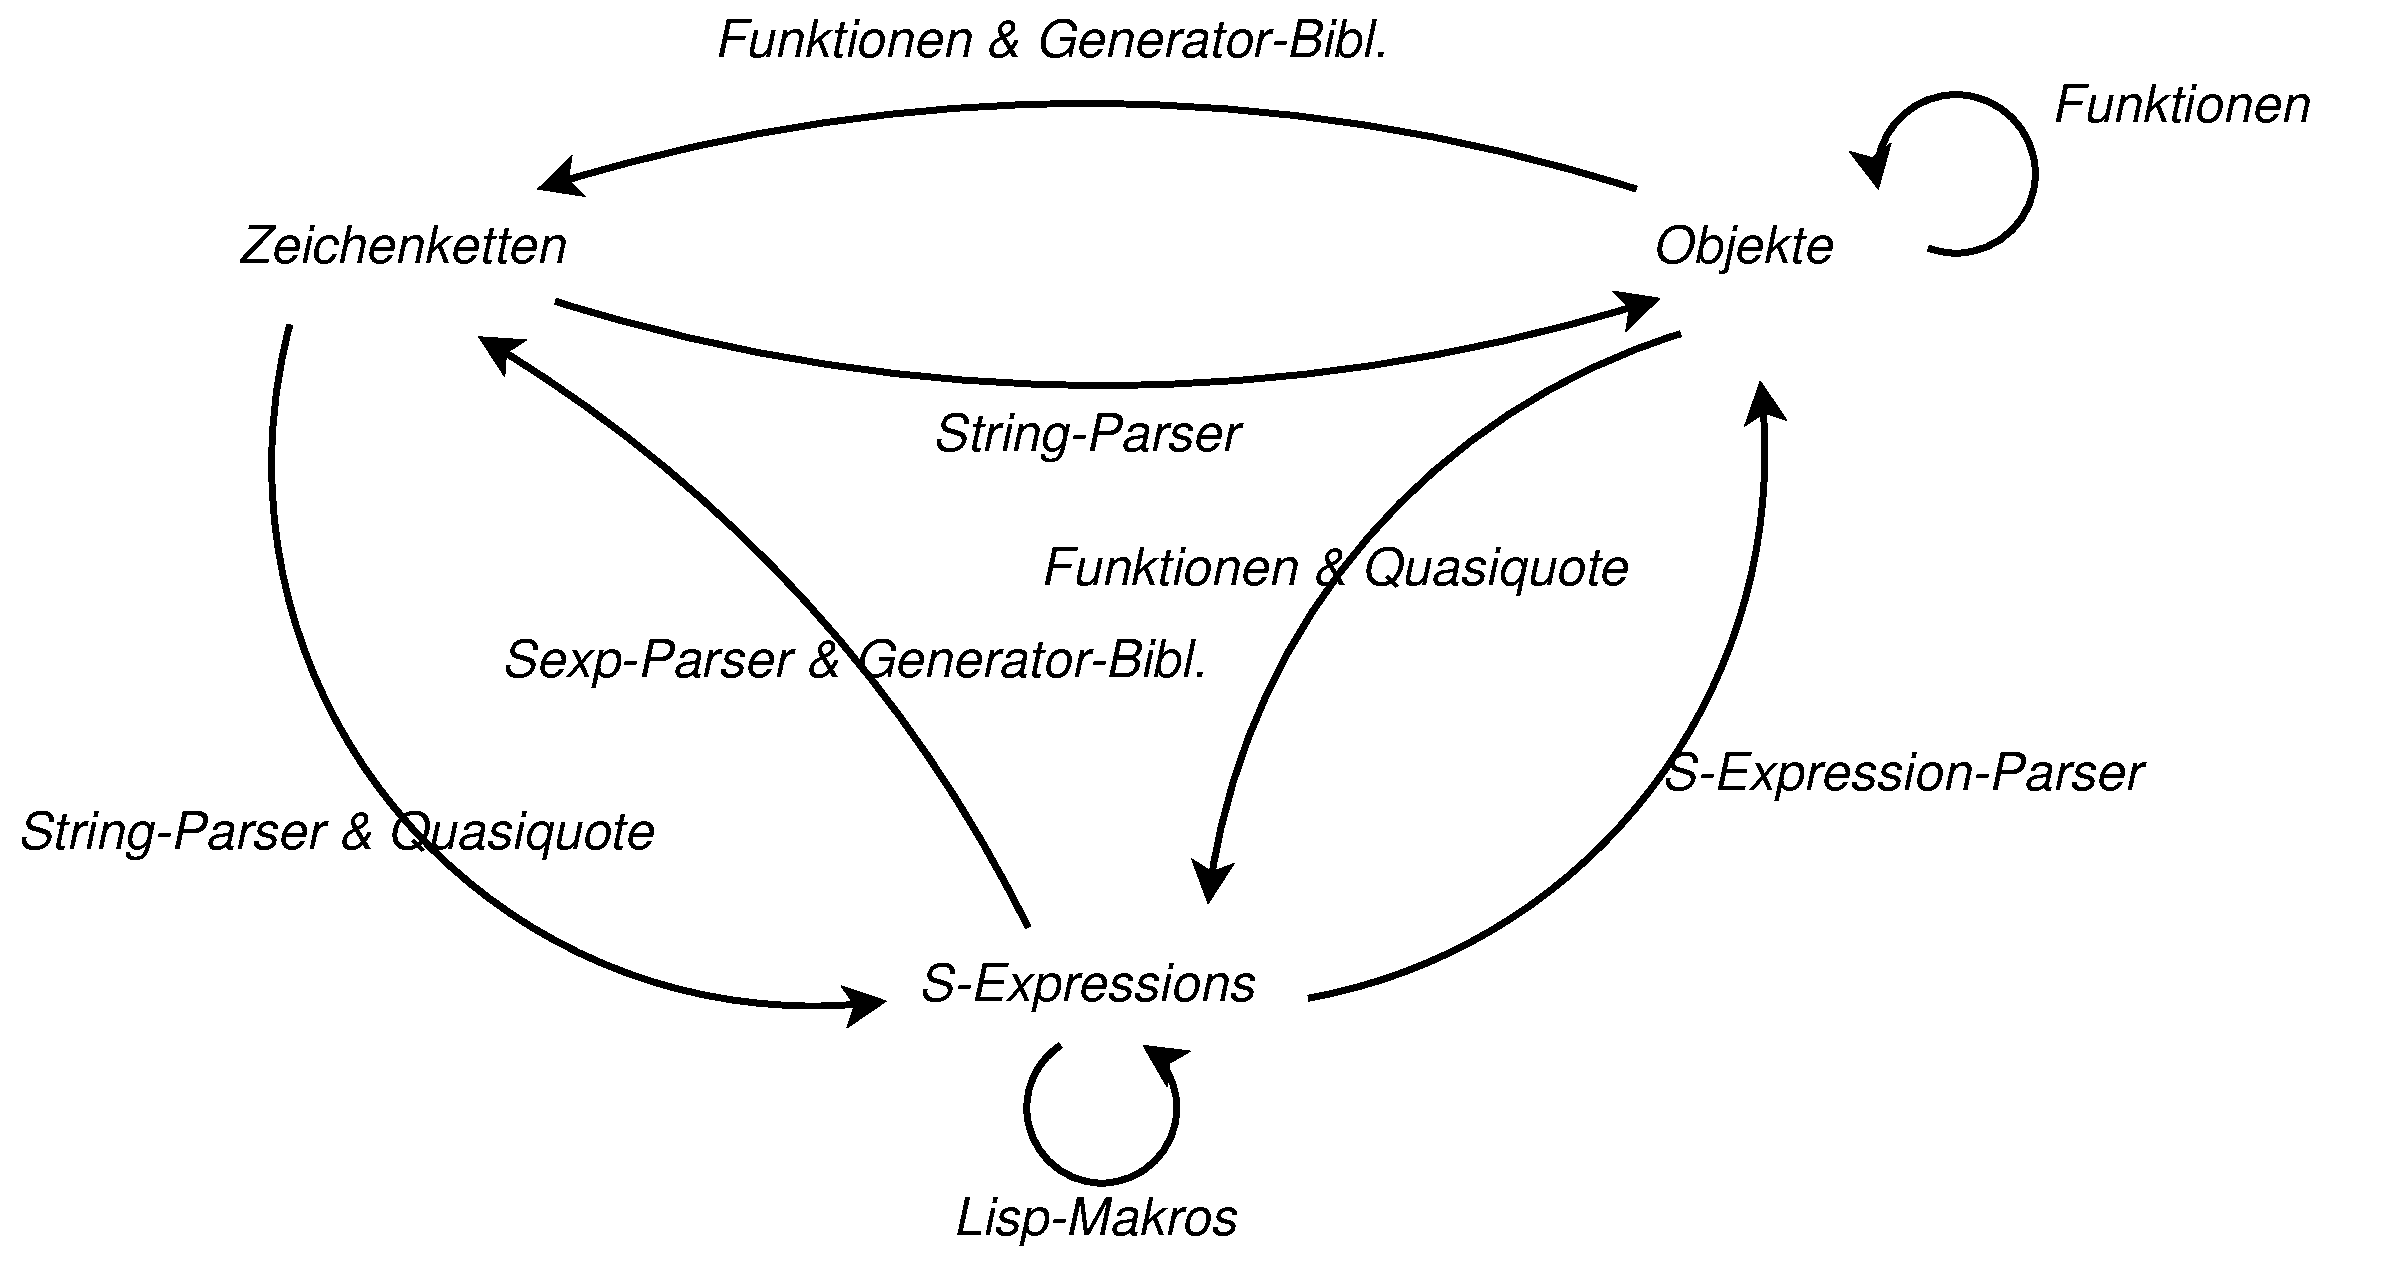
\includegraphics[scale=0.18]{images/magicl_model_support}
    \end{column}
  \end{columns}
\end{frame}

\begin{frame}{Bereitgestellte DSLs}
  \begin{itemize}
  \item Haskell-DSL
    \begin{itemize}
    \item Funktionale \sexp{}-Sprache
    \item ``geklammerte Haskell-Version''
    \item Als Metasprache verwendet
    \item Nach Haskell übersetzt
    \end{itemize}
  \item Compiler-DSL
    \begin{itemize}
    \item Für Compiler-Definitionen
    \item Beinhaltet
      \begin{itemize}
      \item Quasiquote
      \item Lisp-Makros
      \item Haskell-DSL
      \end{itemize}
    \item Nach Haskell-DSL übersetzt
    \end{itemize}      
  \end{itemize}
\end{frame}

\begin{frame}[fragile]{Haskell-DSL-Beispiel}
  \begin{columns}
    \begin{column}{5cm}
      \begin{block}{Haskell-DSL-Code}
\begin{verbatim}
(= (sumOfSquares x y)
   (+ x2 y2)
  (where
    (= x2 (* x x))
    (= y2 (* y y))))  
\end{verbatim}
      \end{block}
    \end{column}
    \begin{column}{6cm}
      \begin{block}{Erzeugter Haskell-Code}
\begin{verbatim}
sumOfSquares x y = (x2 + y2)
  where
    x2 = (x * x)            
    y2 = (y * y)
\end{verbatim}
      \end{block}
    \end{column}
  \end{columns}
\end{frame}

\begin{frame}[fragile]{Übersetzung der Haskell-DSL}
  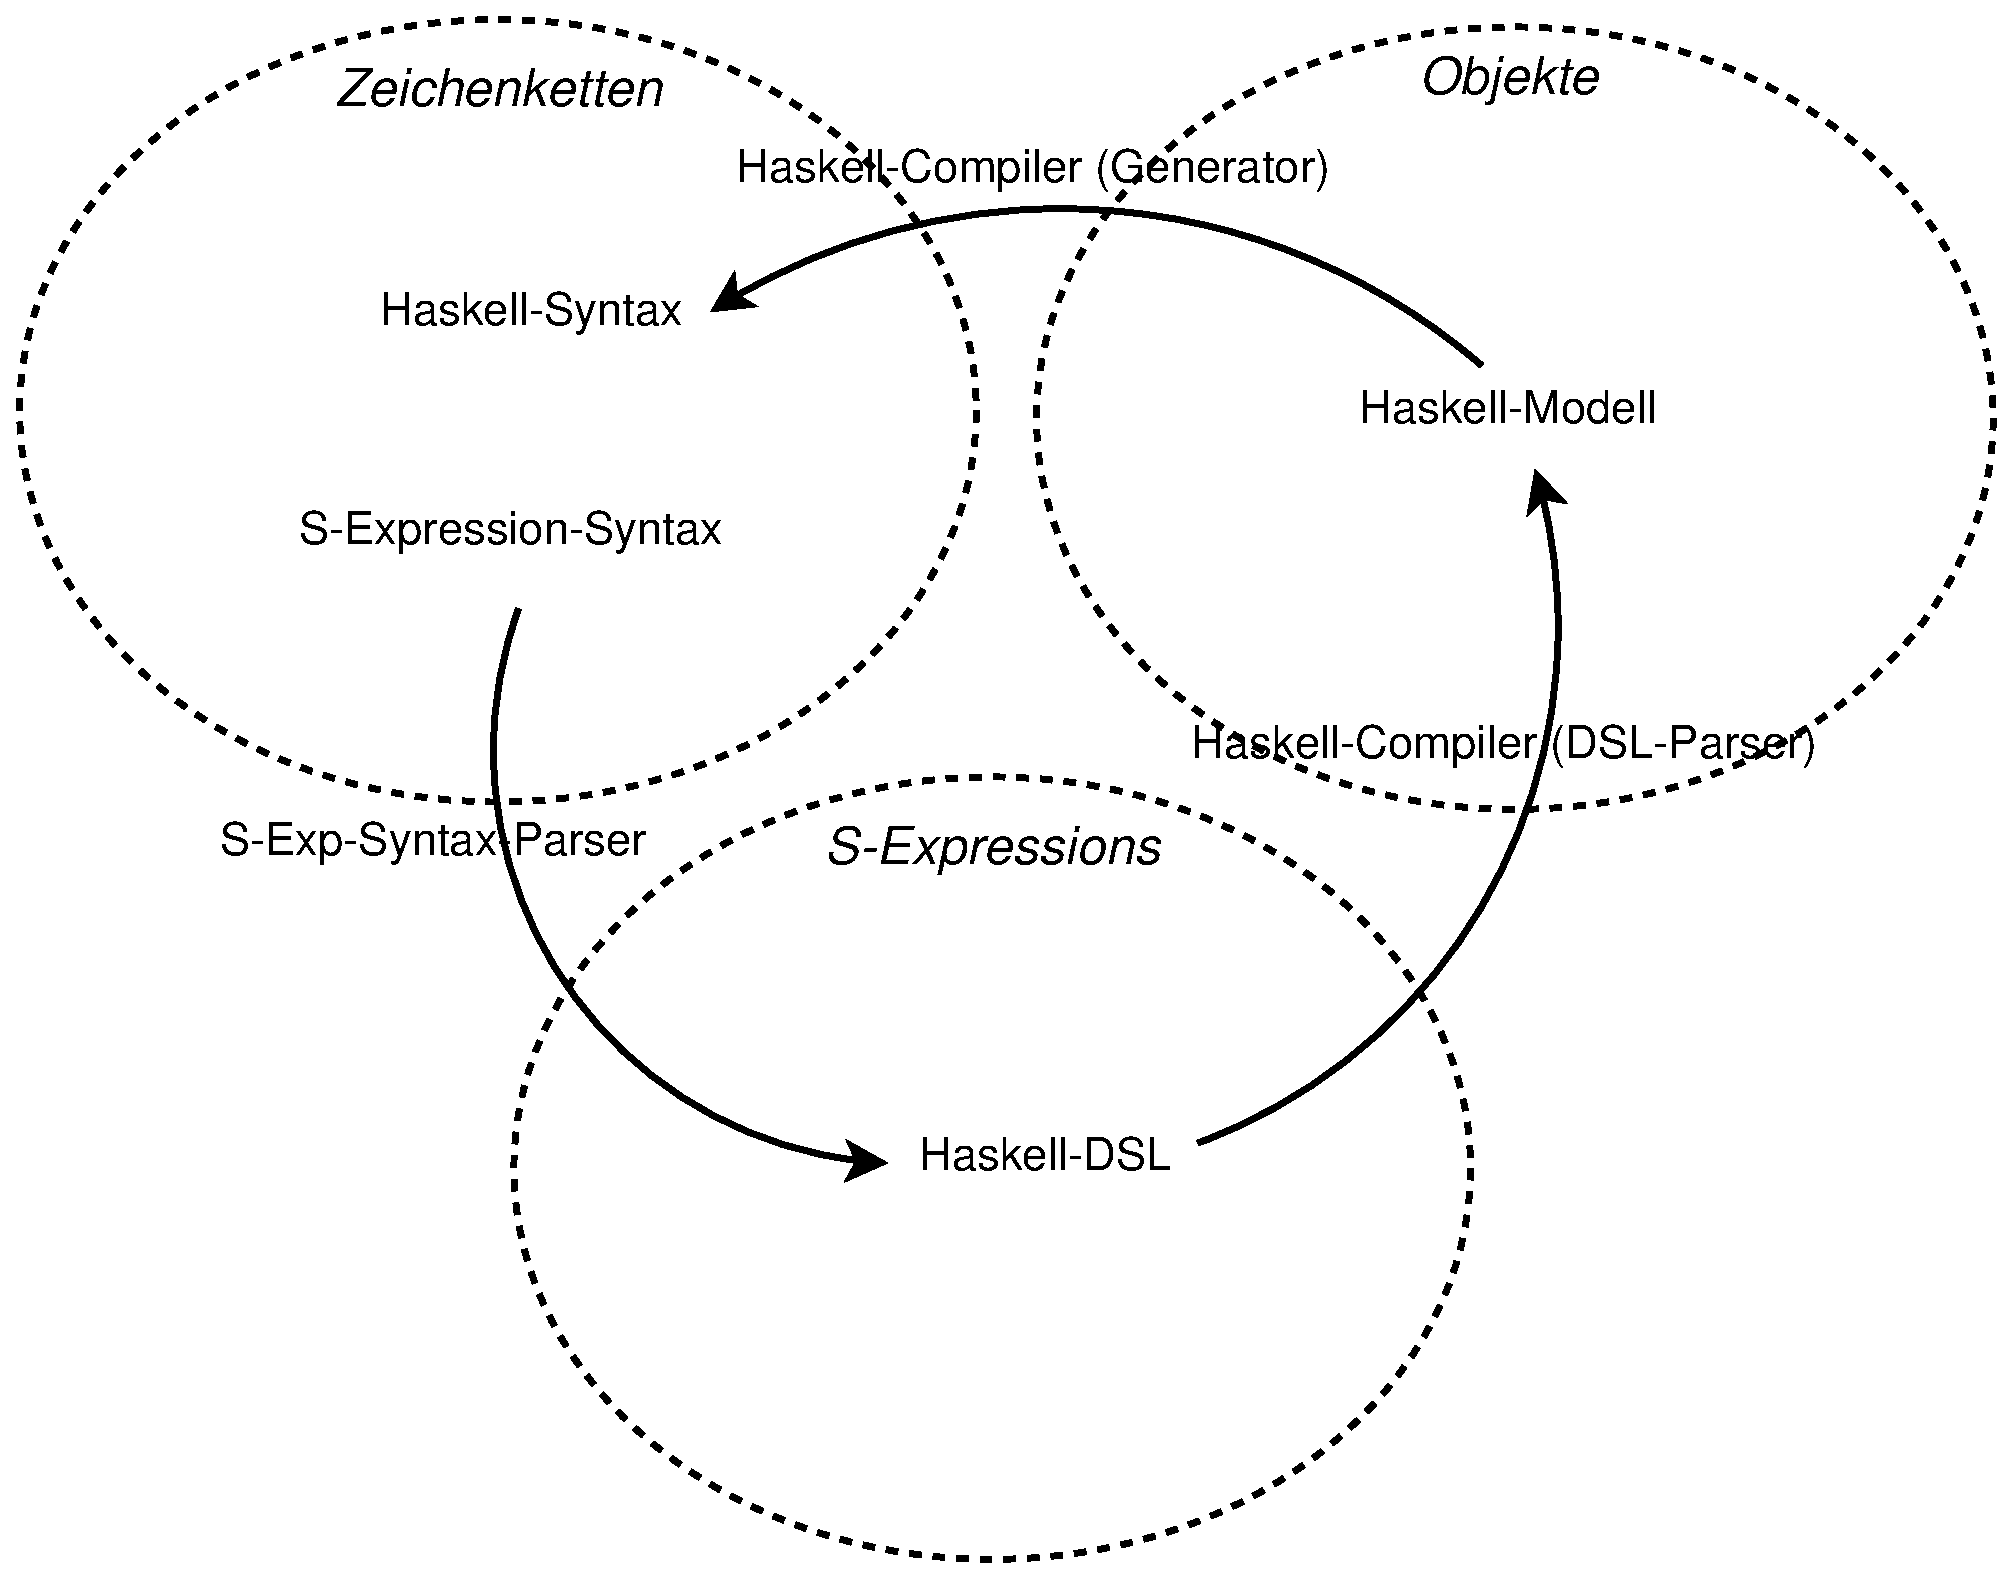
\includegraphics[scale=0.26]{images/magicl_hask_compiler}
\end{frame}

\begin{frame}{Übersetzung der Compiler-DSL}
  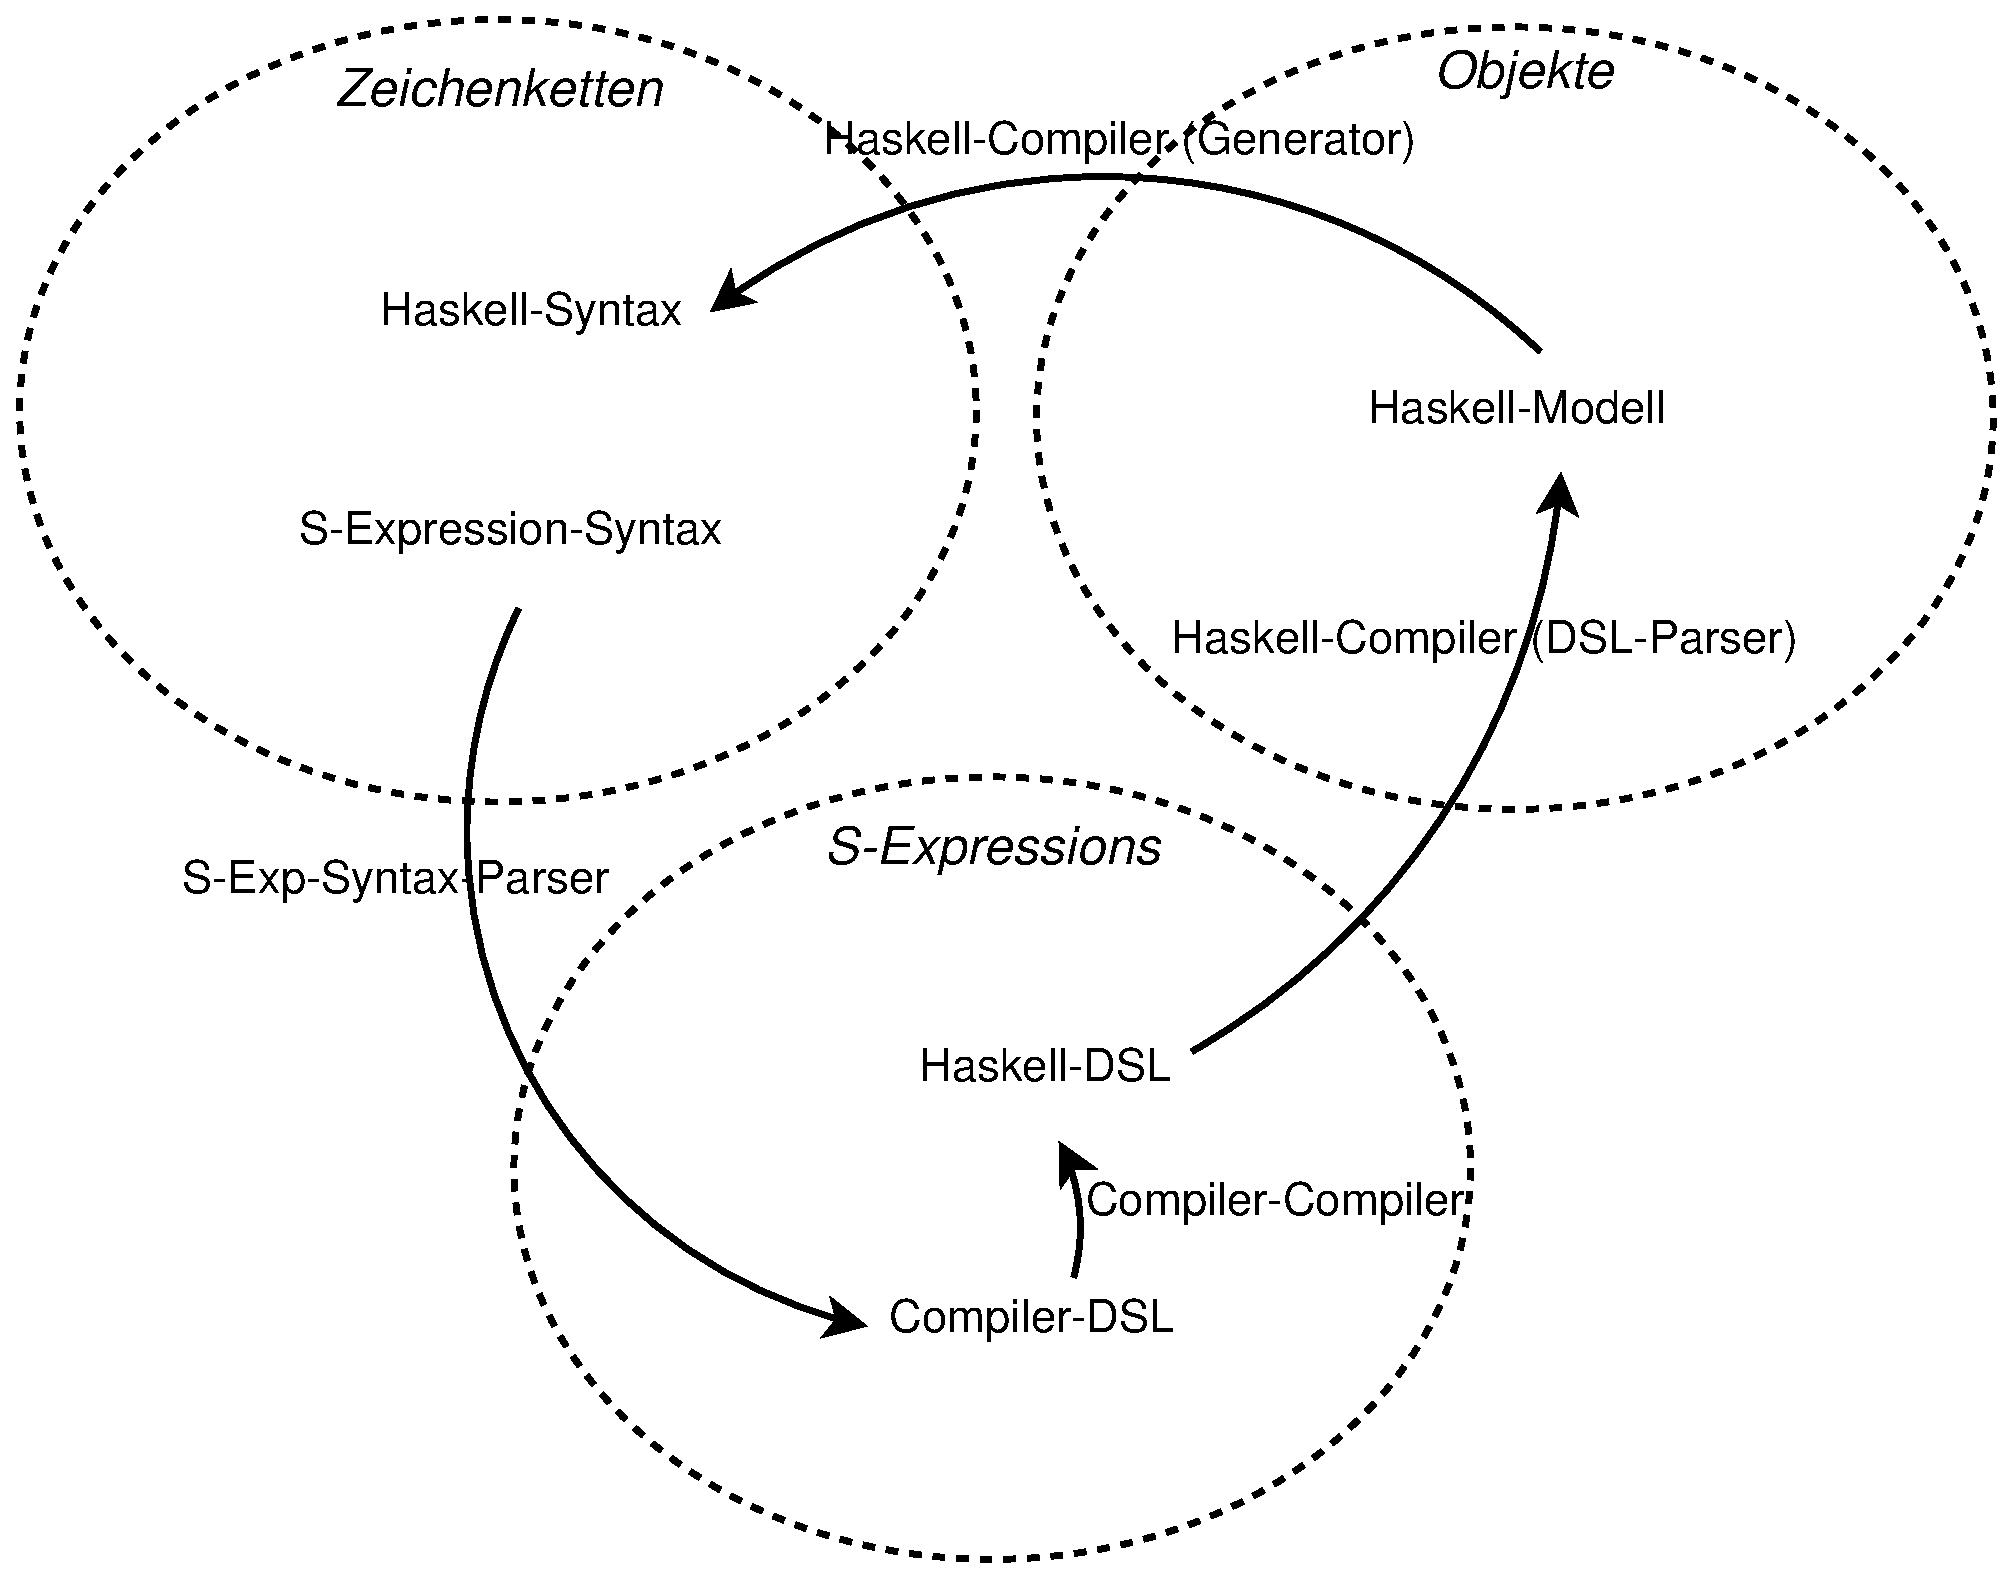
\includegraphics[scale=0.26]{images/magicl_comp_compiler}
\end{frame}

\begin{frame}[fragile]{Parser-Bibliothek}
  \begin{itemize}
  \item Konstruktoren
    \begin{itemize}
    \item \verb+empty+
    \item \verb+eq+
    \item \verb+member+
    \item ...
    \end{itemize}
  \item Kombinatoren
    \begin{itemize}
    \item \verb+many+
    \item \verb+optional+
    \item ...
    \end{itemize}
  \end{itemize}
\end{frame}

\begin{frame}[fragile]{Generator-Bibliothek}
  \begin{itemize}
  \item Funktionale Erzeugung von Code
  \end{itemize}
  \begin{block}{Beispiel}
\begin{verbatim}
  layout 80 (braces 
  (indent2 
  (lines [text "foo",
    words [text "hello", text "world"],
    commaSep [text "1", text "2", text "3"]])))
\end{verbatim}
  \end{block}
  \begin{block}{Erzeugter Code}
\begin{verbatim}
  {foo
    hello world
    1, 2, 3}
\end{verbatim}
  \end{block}
\end{frame}

\begin{frame}{Weitere Komponenten}
  \begin{itemize}
  \item kleines Test-Framework
  \item Build-Tool
  \end{itemize}
\end{frame}

\section{Demo}
\subsection{Demo}

\begin{frame}{Demo}
  \begin{columns}
    \begin{column}{4cm}
      \begin{itemize}
      \item Slide-DSL
      \pfeil Latex-DSL
      \pfeil Latex-Code
      \end{itemize}
    \end{column}
    \begin{column}{6cm}
      \begin{figure}
        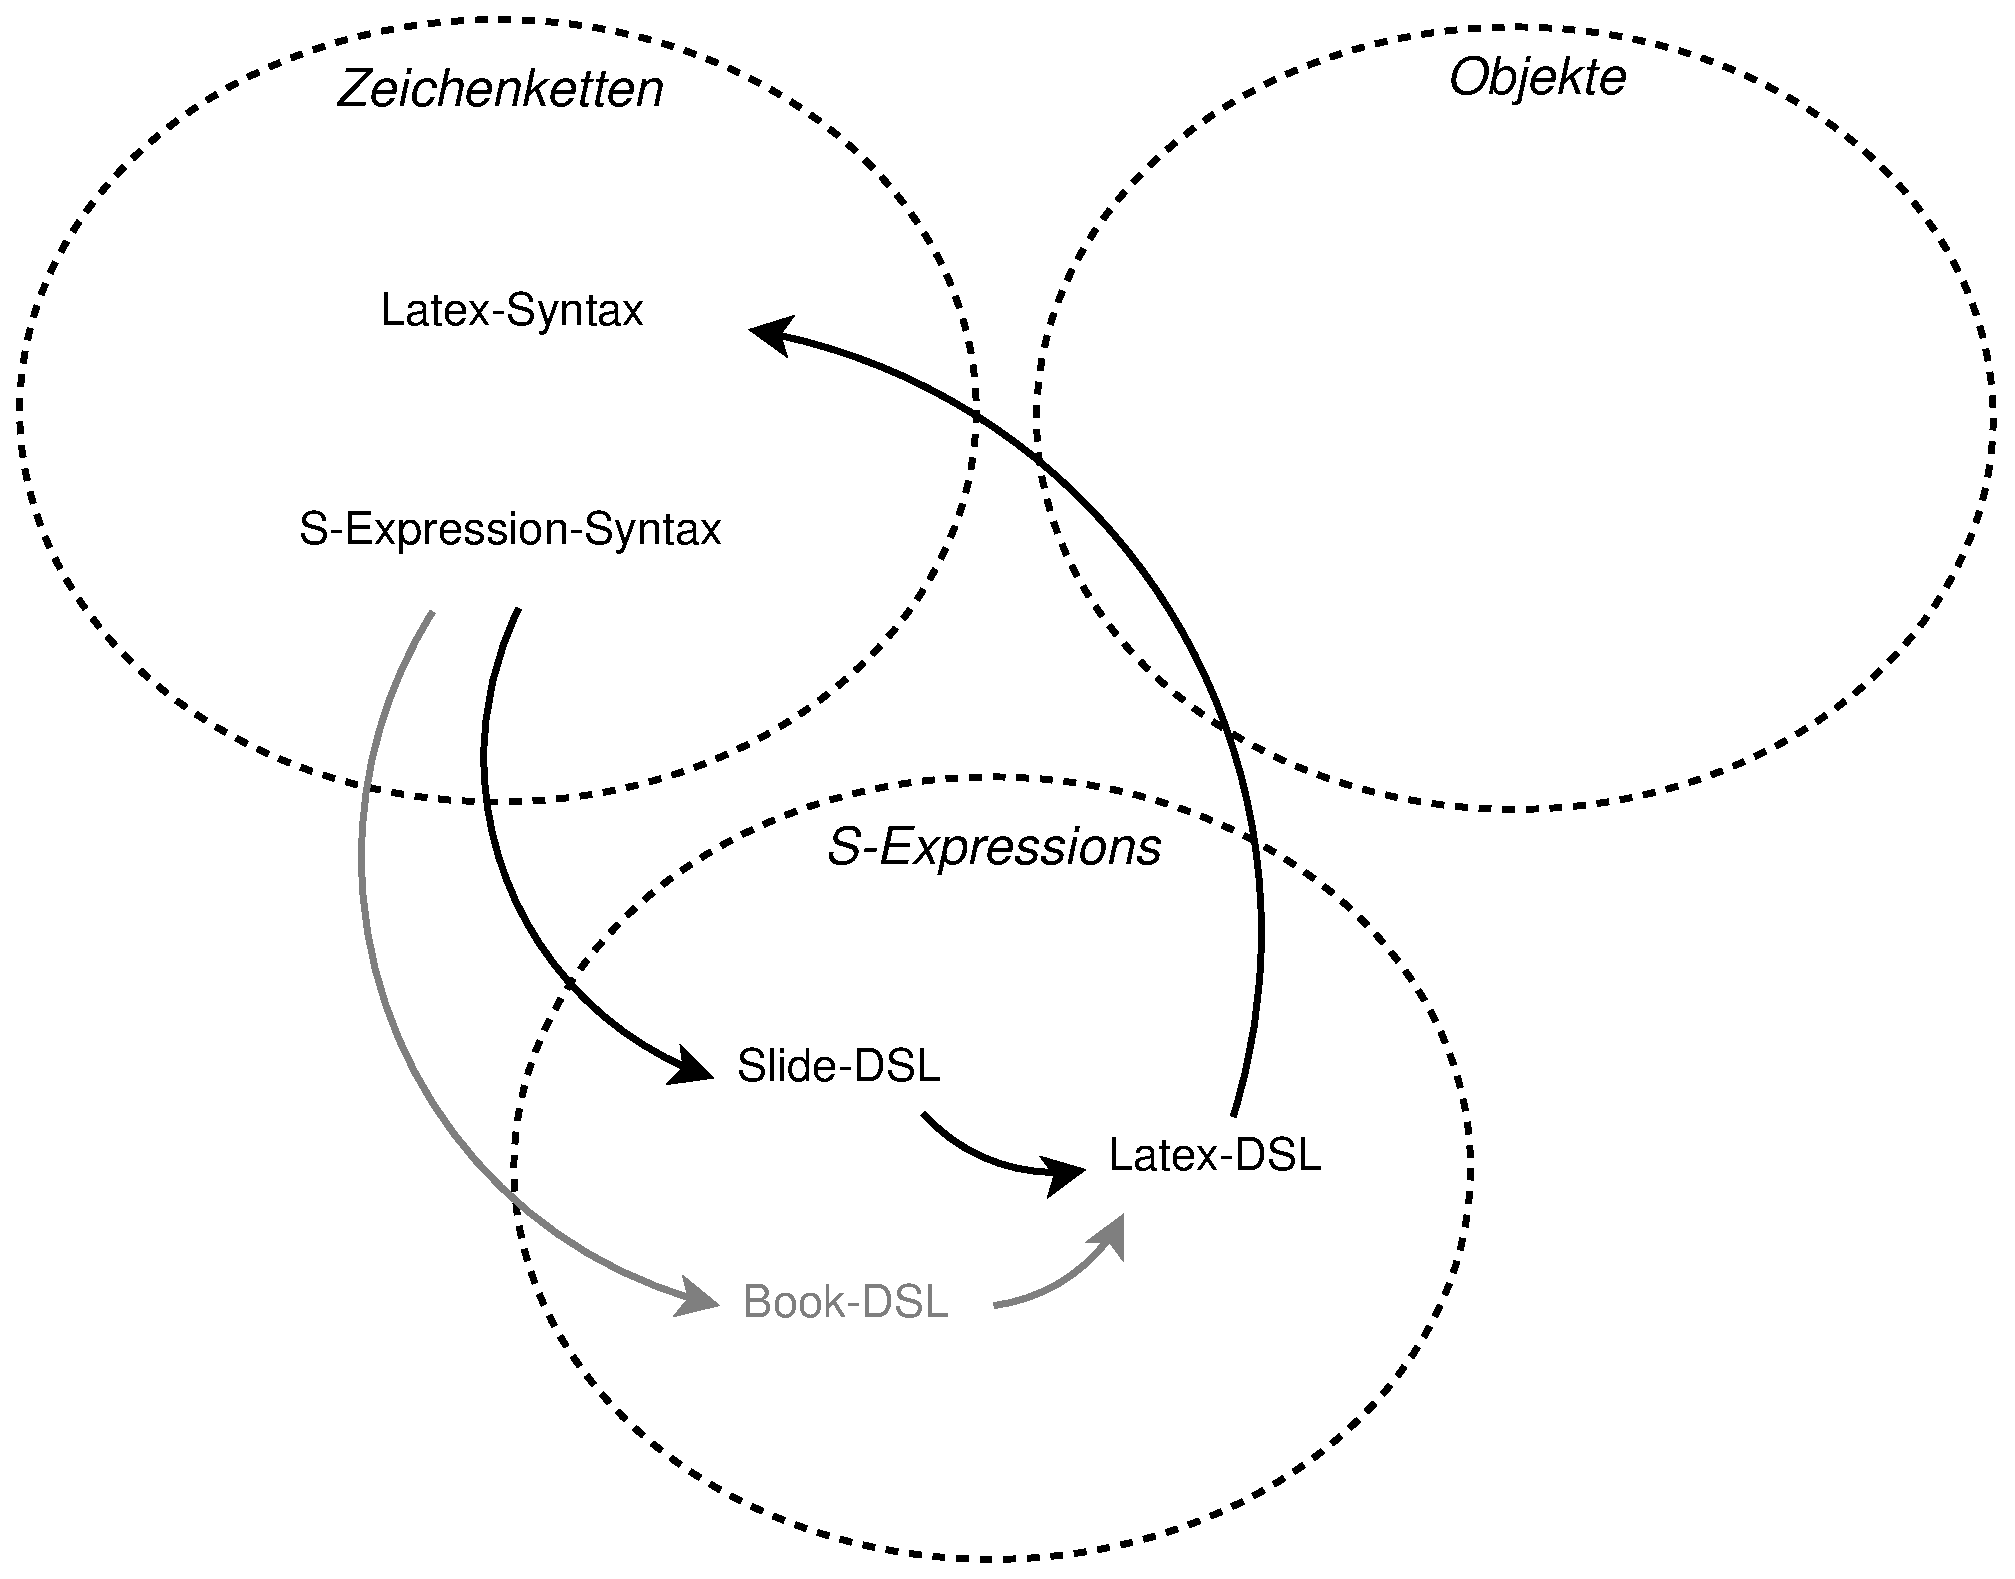
\includegraphics[scale=0.2]{images/magicl_latex_compiler}
        \caption{Übersetzung der Slide-DSL}    
      \end{figure}
    \end{column}
  \end{columns}
\end{frame}

\section{Schluss}
\subsection{Schluss}

\begin{frame}{Zusammenfassung}
  \begin{itemize}
  \item Prototyp eines universellen Compiler-Frameworks
  \item Lisp-inspiriert: \sexps{}, Makros
  \item Architektur
    \begin{itemize}
    \item Haskell
    \item Kategorientheorie
    \end{itemize}
  \item Verallgemeinerungen gegenüber Lisp
    \begin{itemize}
    \item Modelltypen
    \item Verarbeitungsprozesse
    \item Kontrollfluss
    \end{itemize}
  \end{itemize}
\end{frame}

\begin{frame}{Fazit}
  \begin{itemize}
  \item Themengebiet sehr interessant
  \item Framework funktioniert
  \item Manches noch etwas umständlich
    \begin{itemize}
    \item Preis für Verallgemeinerung
    \item Kann durch \cgen{} vereinfacht werden
    \end{itemize}
  \end{itemize}
\end{frame}

\begin{frame}{Ausblick}
  \begin{itemize}
  \item Implementierung sehr komplex
    \begin{itemize}
    \pfeil nächstes Mal KISS-Prinzip!
    \end{itemize}
  \item Einfacher: selbst ein Lisp verwenden
    \begin{itemize}
    \item Bekannte Lisps wirkten veraltet und unsauber
    \item Inzwischen gibt es Clojure!
    \end{itemize}
  \end{itemize}
\end{frame}

\begin{frame}
  \begin{center}
    \Huge Vielen Dank für ihre Aufmerksamkeit!
  \end{center}
\end{frame}

\end{document}
